\section{Implementing the Semi-Supervised VAE (SSVAE)}

So far we have dealt with generative models in the unsupervised setting. We now consider semi-supervised learning on the 
MNIST dataset, where we have a small number of labeled $\bx_{\ell} = {\{(\bx^{(i)},y^{(i)})\}}_{i=1}^{100}$ pairs in our 
training data and a large amount of unlabeled data $\bx_{u} = {\{\bx^{(i)}\}}_{i=101}^{60000}$. A label $y^{(i)}$ for an 
image is simply the number the image $\bx^{(i)}$ represents. We are interested in building a classifier that predicts the 
label $y$ given the sample $\bx$. One approach is to train a classifier using standard approaches using only the labeled data. 
However, we would like to leverage the large amount of unlabeled data that we have to improve our classifier’s performance.

We will use a latent variable generative model (a VAE), where the labels $y$ are partially observed, and $\bz$ are always unobserved. 
The benefit of a generative model is that it allows us to naturally incorporate unlabeled data into the maximum likelihood 
objective function simply by marginalizing $y$ when it is unobserved. We will implement the Semi-Supervised VAE (SSVAE) 
for this task, which follows the generative process specified below:

\begin{equation}\label{eq:15}
    p(\bz) = \calN(\bz \mid 0, I)
\end{equation}


\begin{equation} \label{eq:16}
    p(y) = \text{Categorical}(y \mid \pi) = \frac{1}{10}
\end{equation}

\begin{equation} \label{eq:17}
    p_{\theta}(\bx \mid y, \bz) = \text{Bern}\left(\bx \mid f_{\theta}\left(y,\bz\right)\right)
\end{equation}

where $\pi = (1/10,...,1/10)$ is a fixed uniform prior over the 10 possible labels and each sequence of pixels $\bx$ is 
modeled by a Bernoulli random variable parameterized by the output of a neural network decoder $f_{\theta}(\cdot)$.

\begin{figure}[h]
    \centering
    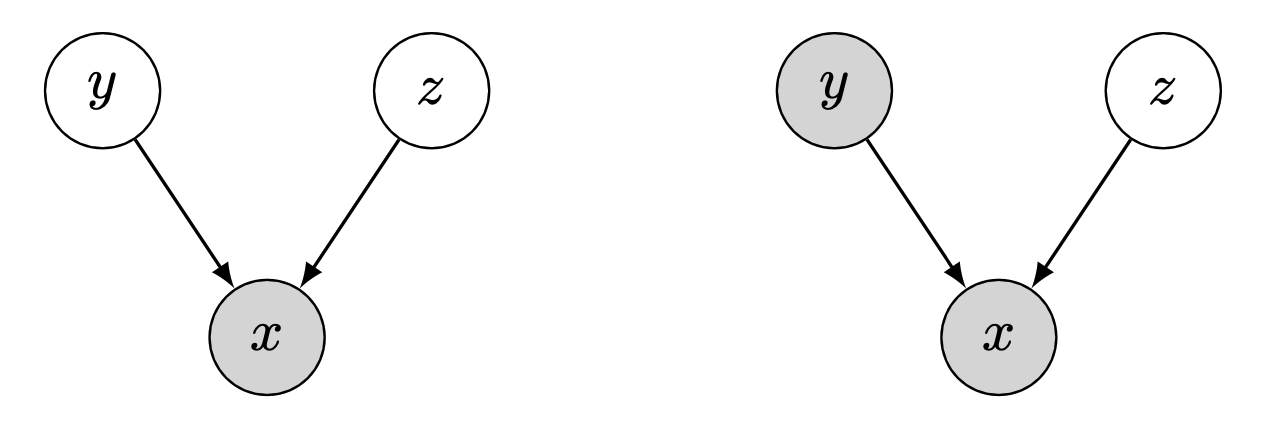
\includegraphics[width=0.3\textwidth]{./figures/ssvae}
    \caption{Graphical model for SSVAE. Gray nodes denote observed variables; unshaded nodes denote latent variables. \textbf{Left}: SSVAE for the setting where the labels $y$ are unobserved; \textbf{Right}: SSVAE where some data points $(x, y)$ have observed labels.}
    \label{fig:ssvae}
\end{figure}

To train a model on the datasets $\bX_{\ell}$ and $\bX_u$, the principle of maximum likelihood suggests that we find the model 
$p_{\theta}$ which maximizes the likelihood over both datasets. Assuming the samples from $\bX_{\ell}$ and $\bX_u$ are drawn i.i.d., 
this translates to the following objective:

\begin{equation} \label{eq:18}
    \max\limits_{\theta} \sum\limits_{x\in\bX_u} \log p_{\theta}(\bx) + \sum\limits_{\bx,y\in\bX_{\ell}} \log p_{\theta}(\bx, y)
\end{equation}

where

\begin{equation} \label{eq:19}
    p_{\theta}(\bx) = \sum\limits_{y \in \calY} \int p_{\theta}(\bx,y,\bz)d\bz
\end{equation}

\begin{equation} \label{eq:20}
    p_{\theta}(\bx, y) = \int p_{\theta}(\bx,y,\bz)d\bz
\end{equation}

To overcome the intractability of exact marginalization of the latent variables $\bz$, we will instead maximize their
respective evidence lower bounds,

\begin{equation}\label{eq:21}
    \max\limits_{\theta, \phi} \sum\limits_{x\in\bX_u} \text{ELBO}(\bx; \theta, \phi) + \sum\limits_{\bx,y\in\bX_{\ell}} \text{ELBO}(\bx, y; \theta, \phi)
\end{equation}

where we introduce some amortized inference model $q_{\phi}(y,\bz \mid \bx) = q_{\phi}(y \mid \bx) q_{\phi}(\bz \mid \bx, y)$. Specifically,

\begin{equation} \label{eq:22}
    q_{\phi}(y \mid \bx) = \text{Categorical}\left(y \mid f_{\phi}\left(\bx\right)\right)
\end{equation}

\begin{equation} \label{eq:23}
    q_{\phi}(\bz \mid \bx, y) = \calN\left(\bz \mid \mu_{\phi}\left(\bx, y\right),\text{diag}\left(\sigma_{\phi}^2\left(\bx, y\right)\right) \right)
\end{equation}

where the parameters of the Gaussian distribution are obtained through a forward pass of the encoder. We note that 
$q_{\phi}(y \mid \bx) = \text{Categorical}(y \mid f_{\phi}(\bx))$ is actually an MLP classifier that is also a part of the 
inference model, and it predicts the probability of the label $y$ given the observed data $\bx$.

We use this amortized inference model to construct the ELBOs.

\begin{equation} \label{eq:24}
    \text{ELBO}(\bx; \theta, \phi) = \E_{q_{\phi}(y,\bz \mid \bx)} \left[\log \frac{p_{\theta}\left(\bx,y,\bz\right)}{q_{\phi}\left(y,\bz \mid \bx\right)}\right]
\end{equation}

\begin{equation} \label{eq:25}
    \text{ELBO}(\bx, \by; \theta, \phi) = \E_{q_{\phi}(\bz \mid \bx, y)} \left[\log \frac{p_{\theta}\left(\bx,y,\bz\right)}{q_{\phi}\left(\bz \mid \bx, y\right)}\right]
\end{equation}

However, Kingma et al. (2014)\footnote{Kingma, et al. Semi-Supervised Learning With Deep Generative Models. Neural Information Processing Systems, 2014} 
observed that maximizing the lower bound of the log-likelihood is not sufficient to learn a good classifier. Instead, they proposed 
to introduce an additional training signal that directly trains the classifier on the labeled data

\begin{equation} \label{eq:26}
    \max\limits_{\theta, \phi} \sum\limits_{x\in\bX_u} \text{ELBO}(\bx; \theta, \phi) + \sum\limits_{\bx,y \in \bX_{\ell}} \text{ELBO}(\bx,y;\theta,\phi) + \alpha \sum\limits_{\bx,y \in \bX_{\ell}} \log q_{\phi}(y \mid \bx)
\end{equation}

where $\alpha \ge 0$ weights the importance of the classification accuracy. In this problem, we will consider a simpler variant of this objective that works just as well in practice,

\begin{equation} \label{eq:27}
    \max\limits_{\theta, \phi} \sum\limits_{x \in \bX} \text{ELBO}(\bx; \theta, \phi) + \alpha \sum\limits_{\bx,y \in \bX_l} \log q_{\phi}(y \mid \bx)
\end{equation}

where $\bX = \{\bX_u, \bX_{\ell}\}$. It is worth noting that the introduction of the classification loss has a natural interpretation as maximizing 
the ELBO subject to the soft constraint that the classifier $q_{\phi}(y\mid\bx)$ (which is a component of the amortized inference model) 
achieves good performance on the labeled dataset. This approach of controlling the generative model by constraining its inference model 
is thus a form of amortized inference regularization\footnote{Shu, et al. Amortized Inference Regularization. Neural Information Processing Systems, 2018.}.

\begin{enumerate}[label=(\alph*)]
    \item \points{4a} Run 
    \begin{verbatim}
        python main.py --model ssvae --train --gw 0
    \end{verbatim}

    To use GPU acceleration run the command below. 

    \begin{verbatim}
        python main.py --model ssvae --train --gw 0 --device gpu
    \end{verbatim}

    The \texttt{gw} flag denotes how much weight to put on the ELBO(x) 
    term in the objective function; scaling the term by zero corresponds to a traditional supervised learning setting 
    on the small labeled dataset only, where we ignore the unlabeled data. Your classification accuracy on the 
    test set after the run completes (30000 iterations) will be reported to \texttt{submission/SSVAE\_0.pkl}. To
    check your accuracy. run:

    \begin{verbatim}
        python grader.py 4a-0-basic
    \end{verbatim}

    \item  \points{4b} Implement the \texttt{negative\_elbo\_bound} function in \texttt{ssvae.py}. Note that the function expects
    as output the negative Evidence Lower Bound as well as its decomposition into the following terms,

    \begin{equation} \label{eq:28}
        - \text{ELBO}(\bx;\theta,\phi) = - \E_{q_{\phi}(y \mid \bx)} \log \frac{p(y)}{q_{\phi}(y \mid \bx)} - \E_{q_{\phi}(y \mid \bx)}\E_{q_{\phi}(\bz \mid \bx, y)}\left(\log \frac{p\left(\bz\right)}{q_{\phi}\left(\bz \mid \bx, y\right)} + \log p_{\theta}\left(\bx \mid \bz, y\right)\right)
    \end{equation}
    \begin{equation} \label{eq:29}
        \underbrace{\KL\left(q_{\phi}\left(y \mid \bx\right) \mid\mid p\left(y\right)\right)}_{\text{KL}_y} + \underbrace{\E_{q_{\phi}(y\mid\bx)}\KL\left(q_{\phi}\left(\bz \mid \bx, y\right) \mid\mid p\left(\bz\right)\right)}_{\text{KL}_z} + \underbrace{\E_{q_{\phi}(y,\bz \mid \bx)} [- \log p_{\theta}(\bx \mid \bz, y)]}_\text{Reconstruction}
    \end{equation}

    Since there are only ten labels, we shall compute the expectations with respect to $q_{\phi}(y \mid \bx)$ exactly, while 
    using a single Monte Carlo sample of the latent variables $\bz$ sampled from each $q_{\phi}(\bz \mid \bx,y)$ when dealing 
    with the reconstruction term. In other words, we approximate the negative ELBO with

    \begin{equation} \label{eq:30}
        \KL\left(q_{\phi}\left(y \mid \bx\right) \mid\mid p\left(y\right)\right) + \sum\limits_{y \in \calY} q_{\phi}(y \mid \bx) \left[\KL\left(q_{\phi}\left(\bz \mid \bx, y\right) \mid\mid p\left(\bz\right)\right) - \log p_{\theta}\left(\bx \mid \bz^{(y)}, y\right)\right]
    \end{equation}

    where $\bz^{(y)} \sim q_{\phi}(\bz \mid \bx, y)$ denotes a sample from the inference distribution when conditioned on a possible
    $(\bx, y)$ pairing. The functions \texttt{kl\_normal} and \texttt{kl\_cat} in \texttt{utils.py} will be useful.

    \item \points{4c} Run 
    \begin{verbatim}
        python main.py --model ssvae --train
    \end{verbatim}

    To use GPU acceleration run the command below.
    \begin{verbatim}
        python main.py --model ssvae --train --device gpu
    \end{verbatim}

    This will run the SSVAE with the ELBO(x) term included, and thus perform 
    semi-supervised learning. Your classification accuracy on the test set after the run completes will be saved to \texttt{submission/SSVAE\_1.pkl}. Your accuracy on the test set should be $> 90\%$.
    To check your accuracy, run:
    \begin{verbatim}
        python grader.py 4c-0-basic
    \end{verbatim}

    \textbf{Note 1: }When training the SSVAE model, if you experience an out-of-control growth on the $KL_{z}$ term,
    please check the inputs into \texttt{ut.kl\_cat}. Try double checking if your inputs are correct (especially the third term). 

    \textbf{Note 2: }If you report a drop of accuracy when training it is most likely as a result of issue with reshaping or summing over the wrong dimension. Make sure you are doing those correctly.
\end{enumerate}